\scanpage{19}
D\unsure{é|è}m. par récurrence, c'est trivial si $\operatorname{card} I=0,1$ Le cas $
% ROOT-G01 / L019-03: complete second card word with one locally qualified point.
% Root source specification: full-scan origin (565,160), x right/y down.
% Fixed local rectangle (0,0)--(150,75); .006cm/source unit; baseline y55.
% Point character, role, hand and surface origin remain unestablished.
% Manual placement only; no rendered or metric validation.
\mathop{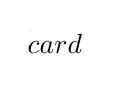
\begin{tikzpicture}[x=.006cm,y=-.006cm,baseline=(root-card-two-base.base)]
\path[use as bounding box] (0,0) rectangle (150,75);
\node[anchor=base west,inner sep=0pt,outer sep=0pt] (root-card-two-base) at (0,55) {$\operatorname{card}$};
\fill[gray!60] (5,6) ellipse (1.2 and 1.2);
\node[inner sep=0pt,outer sep=0pt] at (5,6) {$\unsure{\phantom{\cdot}}$};
\end{tikzpicture}}
 I=2$ a été vu. Cas général \unsure{avec} $\operatorname{card} I\geqslant 3$, on choisit $J$ comme dessus. Il suffit de voir que les ens.
\[
% G01: complete first U, with its three visible entrance/body paths.
% Source origin (580,540), positive x right and y down; unit .009 cm/pixel.
% Baseline at source y=594. Primary reading U with entrance flourish;
% alternative a cancelled equals before U. The role remains unresolved.
\mathord{\unsure{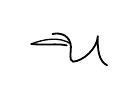
\begin{tikzpicture}[x=.009cm,y=-.009cm,baseline=(g01base.base)]
\path[use as bounding box] (0,0) rectangle (118,60);
\node[anchor=base west,inner sep=0pt,outer sep=0pt] (g01base) at (0,54) {};
\draw[line width=.65pt,line cap=round,line join=round] (35,9) .. controls (48,6) and (60,12) .. (61,27) .. controls (61,36) and (58,46) .. (64,48) .. controls (78,47) and (98,30) .. (99,12) .. controls (98,32) and (101,48) .. (112,53);
\draw[line width=.48pt,line cap=round] (5,23) .. controls (23,16) and (45,12) .. (61,23);
\draw[line width=.65pt,line cap=round] (5,23) .. controls (23,25) and (43,22) .. (55,25);
\end{tikzpicture}|\deleted{=}U}}_{J,i}\cap\Sigma_i^+,\ U_{J,i}\cap\Sigma_i^-
\]
ont la forme précédente, il suffit de le voir pour
\(\underset{\hspace{1.5em}\unsure{\vcenter{\hbox{%
% M01: drawing origin (1124,790) on the full scan; fixed local rectangle.
% The dark point and pale short lower-left trace have undetermined role/hand/origin.
\begin{tikzpicture}[baseline=(0,0),x=0.01cm,y=-0.01cm]
\path[use as bounding box] (0,0) rectangle (42,23);
\fill (35,7) circle[radius=0.02cm];
\draw[gray,line width=0.2pt] (6,18)--(6,20);
\end{tikzpicture}%
}}}}{\text{\unsure{l'une|l'un}}}\)
des deux.

Par hyp. de récurrence, \unsure{on a}
% G03: first footed union, with its rounded inner return and upright retraces.
% Glyph candidates coprod | bigsqcup remain unresolved (original C row R03).
% Source origin (895,965); local rectangle [0,0,125,90]; baseline y=80.
\[
U_{J,i}=X\setminus\mathop{\unsure{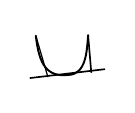
\begin{tikzpicture}[x=0.008cm,y=-0.008cm,baseline=(union-one-base),line cap=round,line join=round]
\coordinate (union-one-base) at (0,80);
\path[use as bounding box] (0,0) rectangle (125,90);
\draw[line width=.7pt] (13,13) .. controls (18,58) and (30,79) .. (65,75) .. controls (93,74) and (94,37) .. (96,12);
\draw[line width=.6pt] (4,80) -- (122,66);
\draw[line width=.45pt] (13,13) -- (32,78);
\draw[line width=.6pt] (96,12) -- (101,71);
\end{tikzpicture}}}\limits_{\alpha\in \overset{\unsure{\cdot}}{\deleted{\unsure{J|\jmath}}}K_0}\widehat{\Sigma}_\alpha^+
\]
% M02: the point over the predecessor has full-scan centre about (989,1047).
% Its attachment is unresolved. The dotless j alternative prevents a second dot.
où
\[
\vcenter{\hbox{\unsure{%
% M03: pale trace left of brace; drawing origin (488,1276), pixel units.
% Its hand, character, role and surface origin remain undetermined.
\begin{tikzpicture}[baseline=(0,0),x=0.01cm,y=-0.01cm]
\path[use as bounding box] (0,0) rectangle (28,40);
\draw[gray!55,line width=0.18pt] (11,3)--(15,4);
\draw[gray!60,line width=0.23pt] (15,6).. controls (23,11) and (20,18)..(22,22)
  .. controls (22,28) and (13,32)..(8,36)--(1,36);
\end{tikzpicture}%
}}}\quad
% ROOT-G02 / L019-18: complete literal brace with its looped middle return.
% Manual source origin (600,1200), x right/y down, .008cm/source unit.
% Fixed rectangle (0,0)--(80,280), baseline local y140.
% Four draw commands preserve three visible runs; the last two meet at (48,172).
% No rendered or metric validation; surrounding aligned entries are outside this group.
\vcenter{\hbox{%
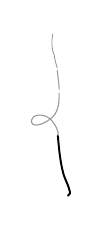
\begin{tikzpicture}[x=.008cm,y=-.008cm,baseline=(root-brace-base.base),line cap=round,line join=round]
\path[use as bounding box] (0,0) rectangle (80,280);
\node[anchor=base west,inner sep=0pt,outer sep=0pt] (root-brace-base) at (0,140) {};
\draw[gray!85,line width=.30pt] (40,10) .. controls (37,23) and (39,37) .. (42,43) .. controls (43,50) and (45,58) .. (47,64);
\draw[gray!75,line width=.40pt] (47,68) .. controls (48,78) and (50,90) .. (50,98);
\draw[gray!80,line width=.40pt] (50,104) .. controls (50,123) and (48,136) .. (36,145) .. controls (20,157) and (5,158) .. (6,147) .. controls (7,138) and (24,135) .. (36,145) .. controls (45,155) and (50,165) .. (48,172);
\draw[line width=.70pt] (48,172) .. controls (50,196) and (52,215) .. (57,233) .. controls (61,245) and (65,251) .. (66,257) .. controls (68,262) and (68,265) .. (64,267);
\end{tikzpicture}%
}}
\begin{aligned}
&\deleted{\Sigma_{\unsure{\alpha|0}}}K_0\subset J\\
&\Sigma_\alpha^+\in\pi_0(X\setminus E_\alpha)\qquad (\forall\,\alpha\in K_0)\\
&\widehat{\Sigma}_\alpha^+=\Sigma_\alpha^+\cup E_\alpha.
\end{aligned}
\]
\unsure{On a|\deleted{O}On a|\deleted{On}On a} donc
% G04: second footed union, inspected independently in half b.
% Same glyph candidates as G03; the first-occurrence uncertainty is printed at G03.
% Source origin (820,1605); local rectangle [0,0,95,93]; baseline y=80.
\[
% The later footed join was independently inspected. Its local coprod/bigsqcup
% alternative remains in the report; the first-occurrence qualification is above.
U=U_{J,i}\cap\Sigma_i^-=\unsure{\cdot}\,X\setminus\left(\mathop{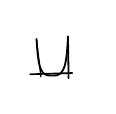
\begin{tikzpicture}[x=0.008cm,y=-0.008cm,baseline=(union-two-base),line cap=round,line join=round]
\coordinate (union-two-base) at (0,80);
\path[use as bounding box] (0,0) rectangle (95,93);
\draw[line width=.65pt] (14,18) .. controls (17,65) and (20,78) .. (40,76) .. controls (61,79) and (62,49) .. (64,14);
\draw[line width=.6pt] (4,74) -- (71,72);
\draw[line width=.45pt] (14,18) -- (21,78);
\draw[line width=.65pt] (64,14) -- (65,80);
\end{tikzpicture}}\limits_{\alpha\in K_0}\widehat{\Sigma}_\alpha^+\ \cup\ \widehat{\Sigma}_i^+\right)
\qquad\underset{\unsure{\vcenter{\hbox{%
% M04: paired dark points; origin (1618,1684) on the full scan.
% These are copied as shapes, without an asserted punctuation or algebraic role.
\begin{tikzpicture}[baseline=(0,0),x=0.01cm,y=-0.01cm]
\path[use as bounding box] (0,0) rectangle (16,19);
\fill (10,6) ellipse[x radius=0.016cm,y radius=0.011cm];
\fill (5,13) ellipse[x radius=0.015cm,y radius=0.011cm];
\end{tikzpicture}%
}}}}{\vphantom{\Sigma}}
\]
% M05: the qualified point preceding X has full-scan centre about (728,1661).
% The second large join retains the first join's qualified primary reading.
\deleted{Soit} Au \unsure{deuxième|deuxieme|dernier} $=$, dans la \deleted{\unsure{somme|réunion}} réunion $\bigcup_{\alpha\in K_0}\widehat{\Sigma}_\alpha^+$, il suffit de se borner \unsure{à|:} sommer sur les \deleted{$\Sigma$} $\alpha\in K_0$ tels que $\widehat{\Sigma}_\alpha^+\not\subset\widehat{\Sigma}_i^+$ i.e. $\Sigma_\alpha^+\not\subset\Sigma_i^+$ soit $K_1$ cet ens., donc
\[
U=X\setminus\left(\bigcup_{\alpha\in K_1}\widehat{\Sigma}_\alpha^+\ \cup\ \widehat{\Sigma}_i^+\right)
\]
% archive sheet number: 18
